\chapter{相对论电动力学}
\label{chap:relativistic electromagnetic}
%三维一般波动方程
%\lapla u-\frac1{a^2}\pv[2]ut=-f(\bm x,t),
%中的$a$是波速,依惯性系而不同。
\paragraph{Michelson-Morley实验}
人们最开始假设光和声音一样,都需要某种介质来支持它的传播。最初假想光是在一种叫作以太(ether)的媒介中传播的,光在相对于以太以不同状态运动时会有不同的速度。为了验证以太是否存在以及光速是否是常数,1887年Michelson和Morley设计了如下所示的光学干涉装置:
\begin{center}
	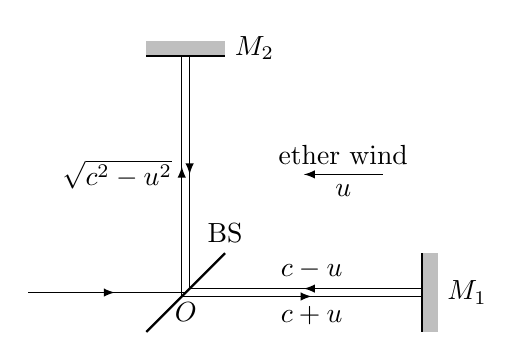
\begin{tikzpicture}
		\draw[-latex](0, 0)--(1.1, 0);
		\draw(1, 0)--(2, 0)node[below]{$O$};
		\draw[thick](2-.5, -.5)--(2.5, .5)node[above]{BS};
		\draw[-latex](2-.05, -.05)--(3.6, -.05)node[below]{$c+u$};
		\draw(3.5, -.05)--(5, -.05);
		\draw(2.05, .05)--(3.6, .05)node[above]{$c-u$};
		\draw[latex-](3.5, .05)--(5, .05);
		\fill[gray!50](5, .5)rectangle(5.2, -.5);
		\node[right]at(5.2, 0){$M_1$};
		\draw[thick](5, .5)--(5, -.5);
		\draw[-latex](2-.05, -.05)--(2-.05, 1.6);
		\draw(2-.05, 1.5)node[left]{$\sqrt{c^2-u^2}$}--(2-.05, 3);
		\draw(2.05, .05)--(2.05, 1.6);
		\draw[latex-](2.05, 1.5)--(2.05, 3);
		\fill[gray!50](1.5, 3)rectangle(2.5, 3.2);
		\node[right]at(2.5, 3.1){$M_2$};
		\draw[thick](1.5, 3)--(2.5, 3);
		\draw[latex-](3.5, 1.5)--(4.5, 1.5)node[midway, below]{$u$}node[midway, above]{ether wind};
	\end{tikzpicture}
	\captionof{figure}{Michelson-Morley光学干涉仪的实验装置图}
	%\label{pic:Michelson-Morley}
\end{center}
图中最左侧相干光源发出的光在经过分束器(beam splitter, BS)中心$O$后,其中一半的光被透射后抵达镜子$M_1$然后被反射回$O$点,另一半的光被反射后抵达镜子$M_2$然后被反射回$O$点,并与从$M_1$反射回来的光发生干涉。假设整个装置在以太中以速度$u$向右运动,那么这等价于装置不动,而以太风以速度$u$向左吹来。%我们可以把“以太风”想象成是一条水流速度为$u$向左均匀流动的河流,把光想象成是一艘固有速度是$c$的船。那么
容易得出光在水平方向从$O$到$M_1$再返回$O$的路径上所花费的时间是:
\[
	T_1=\frac L{c-u}+\frac L{c+u}=\frac{2L/c}{1-u^2/c^2}.
\]
同理,容易得出光在竖直方向上从$O$到$M_2$再返回$O$的路径上所花费的时间是:
\[
	T_2=\frac{2L}{\sqrt{c^2-u^2}}=\frac{2L/c}{\sqrt{1-u^2/c^2}}.
\]
容易发现$T_1\neq T_2$。为了简化计算,假设装置在以太中的运动速度$u\ll c$,那么我们可以对小量做Taylor展开得出光沿着两条路径上传播的时间差是:
\[
	T_1-T_2=\frac{2L}c\biggkh{1+\frac{u^2}{c^2}}-\frac{2L}c\biggkh{1+\frac{u^2}{2c^2}}+\bigo(u^4)=\frac{Lu^2}{c^3}+\bigo(u^4).
\]
由于光沿着两条路径传播存在着如上所示的时间差,即存在所谓光程差,所以我们自然预期在实验观测中会发现光学干涉条纹的偏移。然而,最终的实验结果发现光学干涉条纹并未发生任何改变,%也就是说上述的时间差结果是0!
而且把光学桌旋转一定角度后发现干涉条纹依然没有发生任何改变!这也就从实验上证明了以太并不存在,光速恒为常数$c$!
\section{狭义相对论}
此节仅介绍必要内容,而略去狭义相对论的大部分推导内容。%如尺缩效应、钟慢效应等。
\paragraph{Lorentz变换}
给定惯性系$S$和$S'$,$S'$系相当于$S$系有$x$方向的相对速度$v$,则同一事件(event)在$S,S'$系中的坐标有关系:
%\footnote{为了之后计算方便,也为了更好地凸显出理论的对称性,我们把$c$这个常数定义成1,也就是把光速$c$定义成一个标准单位.这样处理后时间和空间的量纲也统一起来了}
\begin{equation}
	\begin{bmatrix}
		ct'\\x'\\y'\\z'
	\end{bmatrix}=
	\begin{bmatrix}
		\gamma&\gamma\beta\\-\gamma\beta&\gamma\\ &&1\\ &&&1
	\end{bmatrix}
	\begin{bmatrix}
		ct\\x\\y\\z
	\end{bmatrix}
\end{equation}
其中相对速度$\beta\equiv v/c$,Lorentz因子$\gamma\equiv 1/\sqrt{1-\beta^2}$。

如果质点在$S$系中有$x$方向的速度$u=\d x/\d t$,则其在$S'$中的速度为
\begin{equation}
    u'=\dv{x'}{t'}=\frac{\gamma(\d x-v\d t)}{\gamma(\d t-v\d t/c^2)}=\frac{u-v}{1-vu/c^2}.
\end{equation}

\paragraph{四矢量}

为讨论形式的统一,我们定义四矢量(4-vector)。

\begin{definition}{四矢量}{4-vector}
    定义逆变量(contravariant)形如
    \begin{equation}
        a^\mu\equiv(a^0,a^1,a^2,a^3)\tp,
    \end{equation}
    % 称$a^0$是时间(temporal)分量。

    与之对应的是协变量(covariant),形如
    \begin{equation}
        a_\mu\equiv(a_0,a_1,a_2,a_3).
    \end{equation}
\end{definition}
时空连续统(continuum)由位置四矢量表示:
\begin{equation}
    x^\mu\equiv(ct,x,y,z)\tp.
\end{equation}
\begin{definition}{Einstein求和约定}{Einstein summation convetion}
    表达式上下标中出现重复指标时,表示对其遍历求和,即
    \begin{equation}
        a_\mu b^\mu\equiv\sum_\mu a_\mu b^\mu,
    \end{equation}
    因此Einstein约定:这个求和符号是可以省略的。
\end{definition}
% 使用Einstein求和约定,定义四维标量积
% \[
%     a_\mu b^\mu:=a_0b^0+a_1b^1+a_2b^2+a_3b^3\equiv a^\mu b_\mu.
% \]
则Lorentz变换可以表示为
\[
    \bar x^\mu=\Lambda^\mu{}_\nu x^\nu,\quad\Lambda^\mu{}_\nu\equiv
    \begin{bmatrix}
		\gamma&\gamma\beta\\-\gamma\beta&\gamma\\ &&1\\ &&&1
	\end{bmatrix}
\]

\paragraph{时空结构}

狭义相对论时空的具体几何结构由间隔(interval)确定
\[
    s^2(x_A,x_B)=-c^2(t_A-t_B)^2+(x_A-x_B)^2+(y_A-y_B)^2+(z_A-z_B)^2.
\]
可以验证:间隔在Lorentz变换下是不变的:
\footnote{
不变量(invariant)表示在所有惯性系中均保持相同的值;守恒量(conserved quantity)表示在某个过程前后保持相同的值。比如,质量是不变量,却不守恒;能量是守恒的,但不是不变量;电荷量既是不变量,又是守恒量;而速度既不是不变量,也不守恒。

在每个封闭系统中,总的相对论能量和动量都是守恒的。
}
\[
    (s^2)'=-c^2(t_A'-t_B')^2+(x_A'-x_B')^2+(y_A'-y_B')^2+(z_A'-z_B')^2=s^2.
\]
\begin{itemize}
    \item 若$s^2<0$,则称间隔是类时的(timelike),因为这是同地不同时事件间隔的符号;
    \item 若$s^2>0$,则是类空的(spacelike),因为这是同时不同地事件间隔的符号;
    \item 若$s^2=0$,则是类光的(lightlike),因为这是当两个事件由一个以光速传播的信号连接时所保持的关系。
\end{itemize}
在微分形式上,无穷小间隔是
\begin{equation}
    \d s^2=g_{\mu\nu}\d x^\mu\nd x^\nu.
\end{equation}
式中$g_{\mu\nu}$是度规张量(metric tensor)。对于狭义相对论的平坦时空(广义相对论中为弯曲时空),采取Minkowski度规:
\footnote{Minkowski度规有两种:
\begin{itemize}
    \item 东海岸度规$\eta_{\mu\nu}=\diag(-1,1,1,1)$,常用于弦论和宇宙学,其好处是空间分量上的度规分量和我们平时习惯的Euclide空间的度规相同,Griffiths采用此;
    \item 西海岸度规$\eta_{\mu\nu}=\diag(1,-1,-1,-1)$,常用于粒子物理学,Jackson采用此;
    \item 其实还有几乎没人喜欢的$\i ct$。
\end{itemize}
}
\begin{equation}
    g_{\mu\nu}\equiv
    \begin{bmatrix}
        -1\\ &1\\ &&1\\ &&&1
    \end{bmatrix}.
\end{equation}
逆变度规张量$g^{\mu\nu}$应满足
\begin{equation}
    g_{\mu\nu}g^{\nu\rho}=\delta_\mu{}^\rho.
\end{equation}
% 为$g_{\mu\nu}$的归一化余子式。
对平坦时空来说,二者相同$g_{\mu\nu}=g^{\mu\nu}$。

逆变坐标$x_\mu$可由协变坐标$x^\mu$和度规张量得到
\begin{equation}
    x_\mu=g_{\mu\nu}x^\nu.
\end{equation}
同样有$x^\mu=g^{\mu\nu}x_\nu$,写成分量形式就是
\[
    x_0=-x^0,\enspace x_1=x^1,\enspace x_2=x^2,\enspace x_3=x^3.
\]

\paragraph{相对论运动学}

由于钟慢效应(time dilation),在静止系中的时间流速是最慢的,可定义
固有时间(proper time)
\[
    \d\tau=\frac{\d t}{\sqrt{1-u^2/c^2}}\equiv\gamma_u\d t.
\]
进而定义四矢量速度
\begin{equation}
    \eta^\mu\equiv\dv{x^\mu}\tau,
\end{equation}
和四矢量动量
\begin{equation}
    p^\mu\equiv m\eta^\mu.
\end{equation}
其中$m$为(静止)质量。

$p^\mu$的时间分量是$p^0=\gamma_umc$,对应相对论能量:
\[
    E=\gamma_umc^2,
\]
静止时,$\gamma_u=1,\enspace E=mc^2$,二者之差定义为动能
\[
    \Ek\equiv E-mc^2=\frac12mu^2+\frac38\frac{mu^4}{c^2}+\frac5{16}\frac{mu^6}{c^4}+\bigo(u^8),
\]
相对论动量
\[
    \bm p=m\bm\eta=m\dv{\bm x}\tau=\gamma_um\dv{\bm x}t=\gamma_um\bm u.
\]
有关系
\begin{equation}
    E^2=p^2c^2+m^2c^4.
\end{equation}
\begin{example}{Compton散射}{Compton scattering}
    频率为$\nu$的光子与一个静止的电子发生Compton散射,散射后光子的频率变为$\nu'$,散射角为$\theta$,反冲电子动量大小为$p_\elc$,反冲角为$\phi$。
    \begin{center}
        \usetikzlibrary{decorations.pathmorphing}
        \begin{tikzpicture}[>=latex]
            \coordinate (O) at (0, 0);
            \coordinate (x) at (3, 0);
            \coordinate (v) at (3, 2);
            \coordinate (e) at (2, -2);
            \draw[->, thick, gray, decorate, decoration={
                snake, amplitude=.4mm, segment length=2mm, post length=1mm}]
                (-3, 0)node[above]{$h\nu$}--(O);
            \draw[->, thick, decorate, decoration={
                snake, amplitude=.4mm, segment length=4mm, post length=1mm}]
                (O)--(v)node[right]{$h\nu'$};
            \draw[->, thick](O)--(e)node[right]{e$^-$};
            \draw[dashed](O)--(x);
            \pic[draw, "$\theta$", angle radius=8mm, angle eccentricity=1.2]{angle=x--O--v};
            \pic[draw, "$\phi$", angle radius=10mm, angle eccentricity=1.2]{angle=e--O--x};
        \end{tikzpicture}
        \captionof{figure}{Compton散射示意图}
    \end{center}
    由横向、纵向的动量守恒以及能量守恒:
    \begin{subequations}
        \begin{align}
            \frac{h\nu}c&=\frac{h\nu'}c\cos\theta+p_\elc\cos\phi,\\
            0&=\frac{h\nu'}c\sin\theta-p_\elc\sin\phi,\\
            h\nu+m_\elc c^2&=h\nu'+\sqrt{(m_\elc c)^2+(p_\elc c)^2}.
        \end{align}
    \end{subequations}
    解得
    \begin{equation}
        h\nu'=\frac{h\nu}{1+\alpha(1-\cos\theta)},\quad\alpha\equiv\frac{h\nu}{m_\elc c^2}.
    \end{equation}
    将上式改写成波长的形式,得到Compton移动
    \begin{equation}
        \D\lambda=\frac h{m_\elc c}(1-\cos\theta).
    \end{equation}
\end{example}

\paragraph{相对论动力学}

相对论中的力依然遵循Newton第二定律中的定义:
\[
    \bm F\equiv\dv{\bm p}t,
\]
满足
\begin{equation}
    \dv{\bm p}t\cdot\bm u=\dd t\frac{m\bm u}{\sqrt{1-u^2/c^2}}\cdot\bm u=\dv Et.
\end{equation}
因此功能关系:
\begin{equation}
    W\equiv\int\bm F\cdot\d\bm\ell=\int\dv{\bm p}t\cdot\bm u\d t=\D E.
\end{equation}
而Newton第三定律在不同地的时候不再成立,因为在相对论中,同时性是相对的。

可得力在Lorentz变换中的关系
\begin{subequations}
    \begin{align}
        F_x'&=\frac{F_x-v\bm u\cdot\bm F/c^2}{1-vu_x/c^2},\\
        F_y'&=\frac{F_y}{\gamma(1-vu_x/c^2)},\\
        F_z'&=\frac{F_z}{\gamma(1-vu_x/c^2)}.
    \end{align}
\end{subequations}
如果质点在$S$系中保持静止($u=0$),则其受到的力的变换为:
\begin{equation}
    \bm F_\perp'=\frac1\gamma\bm F_\perp,\qquad F_\parallel'=F_\parallel.
\end{equation}
\section{相对论电动力学}
为什么会有磁场?利用静电学和相对论,我们可以计算出载电流线和运动电荷之间的磁力,而不需要援引磁力定律。
\begin{example}{导线的磁场力}{}
    $S$系中有一导线,其中正负电荷线密度为$\pm\lambda$,在导线中反向运动,速度大小为$v$,则正负电荷的线密度大小均为$\lambda=\gamma\lambda_0$,电流为$I=2\lambda v$,导线外距离$r$处有一电荷$q$沿平行于导线的方向以速度$u<v$运动。

    %$S$系中导线没有净电荷,因此电荷$q$不受电场力。
    \begin{center}
        \begin{tikzpicture}[>=latex]
            \draw[->, thick](2, 2.3)--(3, 2.3)node[right]{$\bm v$};
            \draw[->, thick](3, 1.7)--(2, 1.7)node[left]{$-\bm v$};
            \draw[thick](-3, 2)--(3, 2)node[near start, above]{$\lambda$};
            \draw[dashed](0, 0)--(0, 2)node[midway, right]{$r$};
            \draw[->, thick](0, 0)node[left]{$q$}--(.5, 0)node[above]{$\bm u$};
            \fill[black](0, 0)circle(0.1);
        \end{tikzpicture}
        \captionof{figure}{$S$系中导线与电荷示意图}
    \end{center}
    转换到粒子静止的参考系$S'$,则电荷$q$不受磁场力,仅受电场力。
    
    $S'$系中正负电荷的速度为
    \[
        v_\pm=\frac{v\mp u}{1\mp vu/c^2},
    \]
    正负电荷线密度变为$\lambda_\pm=\pm\gamma_{v_\pm}\lambda_0$,总电荷线密度和电场为
    \[
        \lambda\tot=-\frac{2vu}{c^2}\gamma_u\lambda,\quad E=\frac{\lambda\tot}{2\pi\varepsilon_0r}.
    \]
    因此$S'$系中电荷所受的电场力为
    \[
        F'=qE=-\frac{vu\gamma_u\lambda}{c^2}\frac q{\pi\varepsilon_0r}.
    \]
    变回到$S$系中,
    \[
        F=\frac1{\gamma_u}F'=-\frac{vu\lambda}{c^2}\frac q{\pi\varepsilon_0r}=-qu\frac{\mu_0I}{2\pi}.
    \]
    而$S$系中导线没有净电荷,$q$不受电场力,故此力只能是磁场力!
\end{example}
\paragraph{场的变换}
假设:
\begin{compactenum}
	\item 电荷是不变的;
	\item 无论场是如何产生的,转换规则都是相同的。
\end{compactenum}
得到
\begin{align}
    E_x'&=E_x,&E_y'&=\gamma(E_y-vB_z),&E_z'&=\gamma(E_z+vB_y);\\
    B_x'&=B_x,&B_y'&=\gamma\Bigkh{B_y+\frac v{c^2}E_z},&B_z'&=\gamma\Bigkh{B_z-\frac v{c^2}E_y}.
\end{align}
\begin{example}{匀速运动电荷的场}{E, B of q with v}
    考虑$S'$系中,电荷是静止的,没有磁场只有电场:
    \[
        E'=\frac1{4\pi\varepsilon_0}\frac q{r'^2}\uvec r',
    \]
    变换到原系$S$:
    \[
        E_x=E_x',\quad E_y=\gamma E_y',\quad E_z=\gamma E_z',
    \]
    得到电场为$\uvec r$方向,但并不各向同性:
    \begin{equation}
        \bm E=\frac1{4\pi\varepsilon_0}\frac{1-\beta^2}{(1-\beta^2\sin^2\theta)^{3/2}}\frac q{r^2}\uvec r.
    \end{equation}
    磁场为$\uvec\phi$方向:
    \begin{equation}
        \bm B=\frac{\bm v}{c^2}\times\bm E=\frac{\mu_0}{4\pi}\frac{(1-\beta^2)\sin\theta}{(1-\beta^2\sin^2\theta)^{3/2}}\frac{qv}{r^2}\uvec\phi.
    \end{equation}
\end{example}
\subsection{电磁场张量}
电磁场的变换是由一个反对称的二阶张量连接起来的
\[
    t^{\mu\nu}=
    \begin{bmatrix}
        0&t^{01}&t^{02}&t^{03}\\
        -t^{01}&0&t^{12}&t^{13}\\
        -t^{02}&-t^{12}&0&t^{23}\\
        -t^{03}&-t^{13}&-t^{23}&0
    \end{bmatrix}.
\]
变换为 
\[
    \bar t^{\mu\nu}=\Lambda^\mu{}_\rho\Lambda^\nu{}_\sigma t^{\rho\sigma}.
\]
对应分量的变换规则为
\begin{align*}
    \bar t^{01}&=t^{01},&\bar t^{02}&=\gamma(t^{02}-\beta t^{12}),&\bar t^{03}&=\gamma(t^{03}+\beta t^{31}),\\
    \bar t^{23}&=t^{23},&\bar t^{31}&=\gamma(t^{31}+\beta t^{03}),&\bar t^{12}&=\gamma(t^{12}-\beta t^{02}).
\end{align*}
与场变换比较,可得电磁张量
\begin{equation}
    F^{\mu\nu}=
    \begin{bmatrix}
        0&E_x/c&E_y/c&E_z/c\\
        -E_x/c&0&B_z&-B_y\\
        -E_y/c&-B_z&0&B_x\\
        -E_z/c&B_y&-B_x&0
    \end{bmatrix}.
\end{equation}
或对偶(dual)张量
\begin{equation}
    G^{\mu\nu}=
    \begin{bmatrix}
        0&B_x&B_y&B_z\\
        -B_x&0&-E_z/c&E_y/c\\
        -B_y&E_z/c&0&-E_x/c\\
        -B_z&-E_y/c&E_x/c&0
    \end{bmatrix}.
\end{equation}
\paragraph{张量符号中的电动力学}
用张量的语言重新表述电动力学定律(Maxwell方程和Lorentz力)。统一电荷源$\rho$和电流源$\bm J$,定义四矢量电流源
\begin{equation}
    J^\mu=(c\rho,J_x,J_y,J_z)\tp,
\end{equation}
\begin{definition}{四维导数}{}
    定义 
    \begin{equation}
        \p_\mu\equiv\pp{x^\mu},\quad\p^\mu\equiv\pp{x_\mu}.
    \end{equation}
    有
    \begin{equation}
        \p_\mu a^\mu=\p_0a^0+\p_1a^1+\p_2a^2+\p_3a^3=\pv{a^0}{x^0}+\pv{a^1}{x^1}+\pv{a^2}{x^2}+\pv{a^3}{x^3}.
    \end{equation}
\end{definition}
连续性方程\eqref{eqn:continuity}变为 
\[
    \p_\mu J^\mu=\pv\rho t+\div\bm J=0,
\]
Maxwell方程组变为 
\begin{subequations}
    \begin{align}
        \p_\nu F^{\mu\nu}&=\mu_0J^\mu,\\
        \p_\nu G^{\mu\nu}&=0.
    \end{align}
\end{subequations}
$\mu=0$给出 
\begin{subequations}
    \begin{align}
        \div\bm E&=\rho/\varepsilon_0,\\
        \div\bm B&=0;
    \end{align}
\end{subequations}
$\mu=1,2,3$给出$x,y,z$分量 
\begin{subequations}
    \begin{align}
        \curl\bm B-\mu_0\varepsilon_0\pv{\bm E}t&=\mu_0\bm J,\\
        \curl\bm E+\pv{\bm B}t&=\bm0.
    \end{align}
\end{subequations}

定义四矢量Minkowski力 
\begin{equation}
    K^\mu:=q\eta_\nu F^{\mu\nu},
\end{equation}
得到Lorentz力的表达式
\[
    \bm F=q(\bm E+\bm u\times\bm B),
\]

\subsection{相对论势}

将标量势和矢量势的定义:
\begin{align*}
    \bm E&=-\nabla\Phi-\pv{\bm A}t,\\
    \bm B&=\curl\bm A,
\end{align*}
展开,可见对称性:
\begin{alignat*}{2}
    E_x&=-\pv\Phi x-\pv{A_x}t,&\qquad B_x&=\pv{A_y}z-\pv{A_z}y,\\
    E_y&=-\pv\Phi y-\pv{A_y}t,&B_y&=\pv{A_z}x-\pv{A_x}z,\\
    E_z&=-\pv\Phi z-\pv{A_z}t,&B_z&=\pv{A_x}y-\pv{A_y}x,
\end{alignat*}

四矢量势
\begin{equation}
    A^\mu:=(\Phi/c,A_x,A_y,A_z)\tp,
\end{equation}
则电磁张量可以写成
\begin{equation}
    F^{\mu\nu}=\p^\mu A^\nu-\p^\nu A^\mu.
\end{equation}
% 注意这里是协变量$x_\mu$,$x_0=-ct$有一个负号。
\begin{example}{匀速运动电荷的场·续}{E, B of q with v, II}
    续\exmref{exm:E, B of q with v},我们用势的方法再做一遍。$S'$系中电荷静止 
    \[
        \Phi'=\frac1{4\pi\varepsilon_0}\frac q{r'},\quad\bm A'=\bm 0,
    \]
    变回$S$系
    \[
        \Phi=\gamma\Phi',\quad A_x=\gamma\frac v{c^2}\Phi',\quad A_y=A_z=0,
    \]
    其中 
    \[
        r'=\sqrt{x'^2+y'^2+z'^2}=\sqrt{\gamma^2x^2+y^2+z^2}.
    \]
    则
    \[
        \bm E=-\nabla\Phi-\pv{\bm A}t=\frac1{4\pi\varepsilon_0}\frac{\gamma q\bm r}{(\gamma^2x^2+y^2+z^2)^{3/2}}.
    \]
\end{example}
利用四矢量势,Maxwell方程组变为
\[
    \p^\mu\p_\nu A^\nu-\p^\nu\p_\nu A^\mu=\mu_0J^\mu,
\]
使用Lorenz规范
\[
    \p_\mu A^\mu=\frac1{c^2}\pv\Phi t+\div\bm A=0.
\]
由此我们得到了Maxwell方程组最简单的形式:
\begin{equation}
    \p^\nu\p_\nu A^\mu=-\mu_0J^\mu.
\end{equation}
